\documentclass[tikz,border=5pt]{standalone}
\usetikzlibrary{decorations.pathmorphing}

\begin{document}

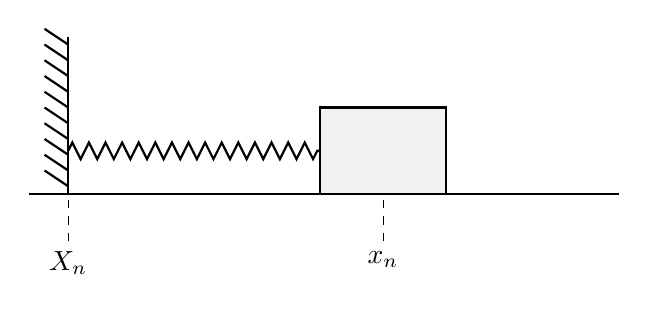
\begin{tikzpicture}[
    spring/.style={thick,decorate,decoration={zigzag,segment length=6,amplitude=3}},
    block/.style={draw,thick,minimum width=1.6cm,minimum height=1.1cm,fill=gray!10}
]

% Floor
\draw[thick] (-0.5,0) -- (7,0);

% Wall
\draw[thick] (0,0) -- (0,2);
\foreach \y in {0.1,0.3,...,1.9}
    \draw[thick] (0,\y) -- (-0.3,\y+0.2);

% Block
\node[block] (B) at (4,0.55) {};

% Spring
\draw[spring] (0,0.55) -- (B.west);

% Wall position marker X
\draw[dashed] (0,-0.6) -- (0,0);
\node[below] at (0,-0.6) {$X_n$};

% Block position marker x
\draw[dashed] (4,-0.6) -- (4,0);
\node[below] at (4,-0.6) {$x_n$};

\end{tikzpicture}

\end{document}